\section{Experiments}
\label{sec:experiments}

\todo{The questions the experiments answer, and the shared evaluation
protocol (trials per task, success criteria).}

\subsection{Real-world tasks}
\label{sec:evaluation-tasks}

The task suite comprises sorting stationery, folding towels, earbuds, and
vegetables from a bag. Figure~\ref{fig:task-success-rates} shows the reporting
layout for task success rates. All plotted numerical values in this draft are
illustrative placeholders pending measured evaluation results.

\begin{figure}[ht]
  \centering
  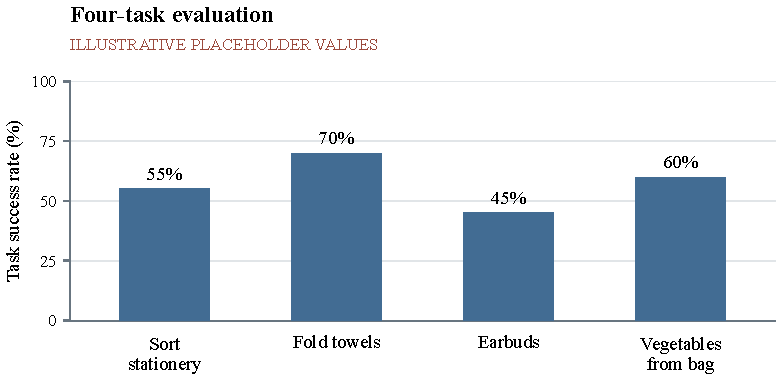
\includegraphics[width=\linewidth]{figures/task_success_rates.pdf}
  \caption{Four-task success-rate plot for sorting stationery, folding towels,
  earbuds, and vegetables from a bag. All plotted numbers are
  \textbf{illustrative placeholder values} and must be replaced
  with measured results before publication.}
  \label{fig:task-success-rates}
\end{figure}

\subsection{Simulation}
\label{sec:simulation-evaluation}

The simulation reporting layout covers Pusher and Grabber. In each setting,
Baseline and ARC are compared under behavior cloning (BC) and co-training,
for both in-domain and generalization cases. Table~\ref{tab:simulation-design}
summarizes the resulting 16 comparison cells.

\begin{table}[ht]
  \centering
  \caption{Simulation comparison design. Each method pair contributes two
  cells, giving 16 cells across settings, evaluation cases, and training regimes.}
  \label{tab:simulation-design}
  \begin{tabular}{@{}llcc@{}}
    \hline
    Setting & Evaluation case & BC & Co-training \\
    \hline
    Pusher & In-domain & Baseline vs.\ ARC & Baseline vs.\ ARC \\
    Pusher & Generalization & Baseline vs.\ ARC & Baseline vs.\ ARC \\
    Grabber & In-domain & Baseline vs.\ ARC & Baseline vs.\ ARC \\
    Grabber & Generalization & Baseline vs.\ ARC & Baseline vs.\ ARC \\
    \hline
  \end{tabular}
\end{table}

Figure~\ref{fig:simulation-comparison} displays this layout as four panels,
with settings arranged by row and evaluation cases by column. Each panel
contains Baseline and ARC bars for BC and co-training. All plotted numbers
are illustrative placeholders pending measured evaluation results; they
support no performance conclusions.

\begin{figure}[htbp]
  \centering
  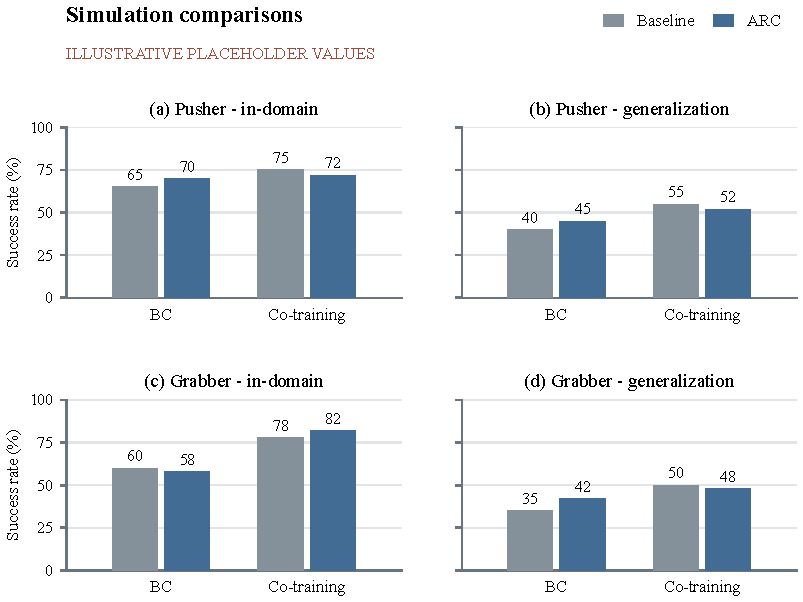
\includegraphics[width=\linewidth]{figures/simulation_comparison.pdf}
  \caption{Simulation comparison layout for Pusher (top) and Grabber (bottom),
  with in-domain cases on the left and generalization cases on the right.
  Each panel compares Baseline with ARC under BC and co-training.
  All plotted numbers are \textbf{illustrative placeholder values} and must
  be replaced with measured results before publication.}
  \label{fig:simulation-comparison}
\end{figure}
